\documentclass{hcmut-report}
\usepackage{codespace}
\usepackage{graphicx}
\usepackage{hyperref}
\usepackage{float}
\usepackage{array}
\usepackage{amsmath}
\usepackage{amssymb}
\usepackage{tikz}
\usetikzlibrary{arrows,automata,positioning,shapes}

\title{Lab 3: Buttons, Debouncing and Traffic Light Controller}
\coursename{Microcontroller}
\reporttype{Lab Report}
\stuname{Âu Lê Quang Trí - 2453300}

\begin{document}
\coverpage

\tableofcontents

\newpage

\section{Introduction and System Architecture}

\subsection{Objectives}
In embedded systems, interfacing digital inputs such as mechanical push-buttons introduces physical challenges (contact bouncing, EMI noise, indeterminate floating states) and architectural challenges (non-blocking event detection, auto-repeat handling, and responsive state navigation). The primary objectives of Laboratory 3 are:
\begin{itemize}
    \item Designing and implementing a robust digital input sampling and software debouncing subsystem on the ARM Cortex-M3 (\textbf{STM32F103C6}).
    \item Building a hierarchical \textbf{Finite State Machine (FSM)} architecture separating input debouncing, user input event dispatching, and high-level traffic control.
    \item Creating a timer-independent software timer module to ensure deterministic execution independent of underlying hardware timer tick rates.
    \item Integrating a four-way crossroad traffic light system complete with 12 traffic LEDs, time-division multiplexed 7-segment displays for dual-road countdowns, and real-time interactive parameter calibration.
\end{itemize}

\subsection{System Overview}
The system models a four-way crossroad controlled by three user push-buttons and displays status across 12 LEDs and four 7-segment displays:
\begin{itemize}
    \item \textbf{Traffic LEDs (12 LEDs total):} The 4-way crossroad contains 4 Red, 4 Amber, and 4 Green LEDs. Road 1 (North--South) and Road 2 (East--West) each govern two opposing traffic heads ($2 \times 3 = 6$ LEDs per road):
    \begin{itemize}
        \item \textbf{Road 1 (North--South, 6 LEDs):} Red 1 (\texttt{PA0}), Amber 1 (\texttt{PA1}), Green 1 (\texttt{PA2}). Both opposing heads operate in parallel.
        \item \textbf{Road 2 (East--West, 6 LEDs):} Red 2 (\texttt{PA3}), Amber 2 (\texttt{PA4}), Green 2 (\texttt{PA5}). Both opposing heads operate in parallel.
    \end{itemize}
    In Proteus simulation, each color pair is represented by one LED indicator per road to maintain a clean schematic while fully simulating the 4-way intersection logic.
    \item \textbf{Multiplexed 7-Segment Displays (4 Digits):}
    \begin{itemize}
        \item Two displays show the countdown time for Road 1 (digits 0 and 1).
        \item Two displays show the countdown time for Road 2 (digits 2 and 3).
        \item Common cathodes $a$--$g$ are tied to a shared bus (\texttt{PB8}--\texttt{PB14}) through $220\,\Omega$ resistors.
        \item Common anodes are driven by external 2N2907 PNP transistors enabled via \texttt{PA6}--\texttt{PA9}.
    \end{itemize}
    \item \textbf{User Push-Buttons (3 Buttons):}
    \begin{itemize}
        \item \textbf{Button 1 (\texttt{PB0}) -- Mode Select:} Cycles the system across 4 operational modes.
        \item \textbf{Button 2 (\texttt{PB1}) -- Value Increment:} Increments active color duration ($1 \to 99\,\text{s}$), supporting single clicks and $500\,\text{ms}$ auto-repeat when held $> 1\,\text{s}$.
        \item \textbf{Button 3 (\texttt{PB2}) -- Set / Commit:} Validates and permanently commits the newly adjusted duration.
    \end{itemize}
\end{itemize}

\subsection{System Operational Modes and the Timing Invariant}
The controller supports four distinct operating modes:
\begin{enumerate}
    \item \textbf{Mode 1 (Normal Operation):} Both roads cycle through standard Green-Amber-Red sequences. Digits 0--1 and 2--3 display synchronous countdown values in seconds.
    \item \textbf{Mode 2 (Modify Red Duration):} All single Red LEDs blink at $2\,\text{Hz}$ ($250\,\text{ms}$ on / $250\,\text{ms}$ off). Digits 2--3 display mode identifier \texttt{02}; digits 0--1 display the red duration under edit.
    \item \textbf{Mode 3 (Modify Amber Duration):} All single Amber LEDs blink at $2\,\text{Hz}$. Digits 2--3 display mode identifier \texttt{03}; digits 0--1 display the amber duration under edit.
    \item \textbf{Mode 4 (Modify Green Duration):} All single Green LEDs blink at $2\,\text{Hz}$. Digits 2--3 display mode identifier \texttt{04}; digits 0--1 display the green duration under edit.
\end{enumerate}

\subsubsection{The Synchronization Invariant Rule}
In a four-way intersection, traffic safety dictates that while Road 1 is Red, Road 2 must complete its entire Green phase and Amber phase before Road 1 can turn Green. Therefore, the durations must strictly satisfy the invariant:
\begin{equation}
    t_{\text{red}} = t_{\text{green}} + t_{\text{amber}}
    \label{eq:time_rule}
\end{equation}
The default factory calibration is configured as:
\begin{equation}
    t_{\text{red}} = 5\,\text{s}, \quad t_{\text{amber}} = 2\,\text{s}, \quad t_{\text{green}} = 3\,\text{s} \quad (5 = 3 + 2)
\end{equation}
Whenever the user modifies one parameter in Modes 2, 3, or 4, the firmware automatically recalculates the dependent parameter upon pressing Button 3 (Set) to maintain equation (\ref{eq:time_rule}) at all times.


\newpage
\section{Exercise 1: Finite State Machine Design}

\subsection{Button Input State Machine}
Mechanical buttons suffer from transient bouncing. Furthermore, user interfaces require distinguishing between a momentary single click and a prolonged press with automatic repeating. 

We model each button as a 3-state FSM inside \texttt{input\_processing.c}:
\begin{itemize}
    \item \textbf{\texttt{BUTTON\_RELEASED}:} Default idle state. When a debounced pressed state is detected, emit a single click event (\texttt{event = 1}) and transition to \texttt{BUTTON\_PRESSED}.
    \item \textbf{\texttt{BUTTON\_PRESSED}:} Button is held down. If released, return to \texttt{BUTTON\_RELEASED}. If held for $\ge 1\,\text{s}$ (\texttt{is\_button\_pressed\_1s()}), advance to the auto-repeat state with a $500\,\text{ms}$ timer.
    \item \textbf{\texttt{BUTTON\_PRESSED\_}\allowbreak\texttt{MORE\_}\allowbreak\texttt{THAN\_}\allowbreak\texttt{1\_SECOND}:} While held, whenever the $500\,\text{ms}$ timer expires, emit a repeat event (\texttt{event = 1}) and reset the timer to $500\,\text{ms}$. If released, return to \texttt{BUTTON\_RELEASED}.
\end{itemize}

\begin{figure}[H]
\centering
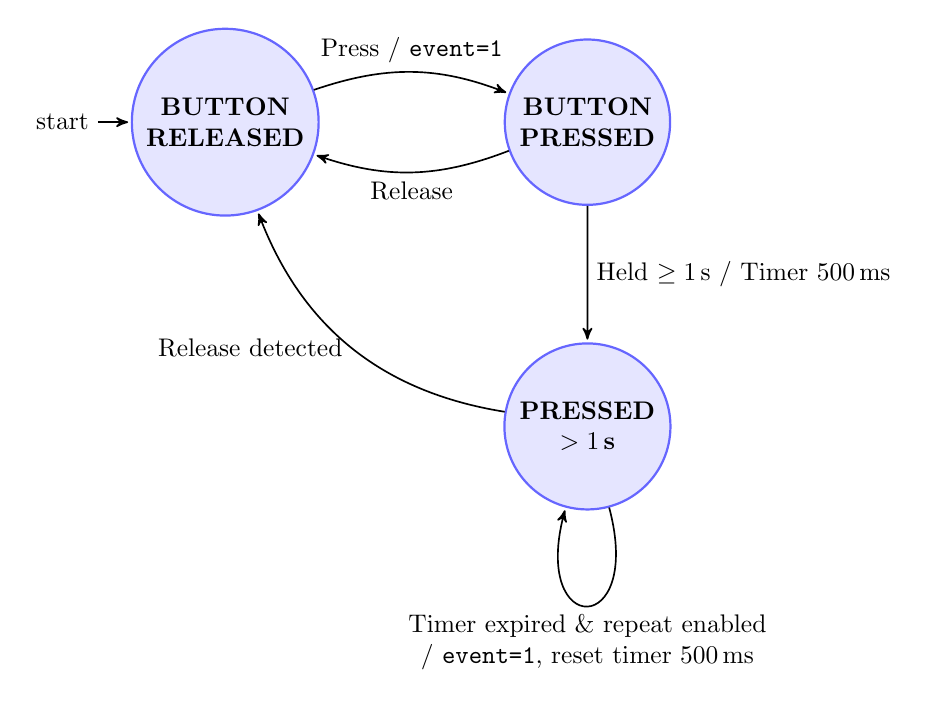
\begin{tikzpicture}[->,>=stealth',shorten >=1pt,auto,node distance=4.5cm,semithick,scale=0.92,every node/.style={transform shape}]
  \tikzstyle{every state}=[fill=blue!10,draw=blue!60,thick,text=black,align=center]

  
\node[initial,state] (A) {\textbf{BUTTON}\\\textbf{RELEASED}};
  
\node[state]         (B) [right of=A, node distance=5.0cm] {\textbf{BUTTON}\\\textbf{PRESSED}};
  
\node[state]         (C) [below of=B, node distance=4.2cm] {\textbf{PRESSED}\\\textbf{$> 1\,\text{s}$}};

  \path (A) edge [bend left=20]  node [above] {Press / \texttt{event=1}} (B)
        (B) edge [bend left=20]  node [below] {Release} (A)
        (B) edge [right]         node [right] {Held $\ge 1\,\text{s}$ / Timer $500\,\text{ms}$} (C)
        (C) edge [bend left=30]  node [left]  {Release detected} (A)
        (C) edge [loop below]    node [below,align=center] {Timer expired \& repeat enabled\\/ \texttt{event=1}, reset timer $500\,\text{ms}$} (C);
\end{tikzpicture}
\caption{Finite State Machine for Button Event Processing with Auto-Repeat}
\label{fig:button_fsm}
\end{figure}

\subsection{Mode Selection Finite State Machine}
The top-level operational state of the traffic controller is governed by a cyclic 4-state Moore machine driven by single-click events from Button 1 (\texttt{PB0}):

\begin{figure}[H]
\centering
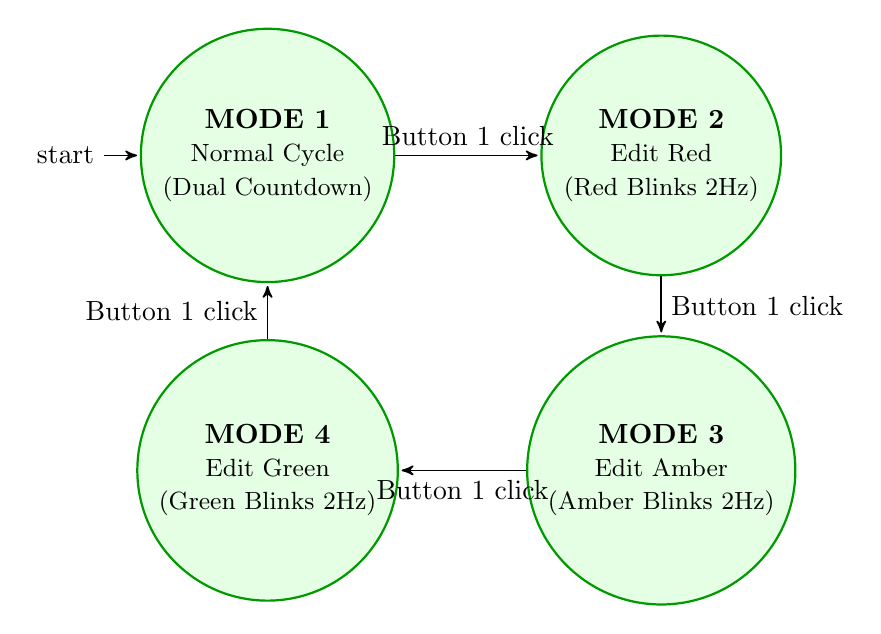
\begin{tikzpicture}[->,>=stealth',shorten >=1pt,auto,node distance=4.2cm,semithick]
  \tikzstyle{every state}=[fill=green!10,draw=green!60!black,thick,align=center]

  
\node[initial,state] (M1) {\textbf{MODE 1}\\\small Normal Cycle\\\small (Dual Countdown)};
  
\node[state]         (M2) [right of=M1, node distance=5cm] {\textbf{MODE 2}\\\small Edit Red\\\small (Red Blinks 2Hz)};
  
\node[state]         (M3) [below of=M2, node distance=4cm] {\textbf{MODE 3}\\\small Edit Amber\\\small (Amber Blinks 2Hz)};
  
\node[state]         (M4) [below of=M1, node distance=4cm] {\textbf{MODE 4}\\\small Edit Green\\\small (Green Blinks 2Hz)};

  \path (M1) edge [above] node {Button 1 click} (M2)
        (M2) edge [right] node {Button 1 click} (M3)
        (M3) edge [below] node {Button 1 click} (M4)
        (M4) edge [left]  node {Button 1 click} (M1);
\end{tikzpicture}
\caption{Top-Level Mode Selection Finite State Machine}
\label{fig:mode_fsm}
\end{figure}

\subsection{Normal Traffic Light 4-Phase Cycle State Machine}
In Mode 1, the traffic intersection executes four consecutive phases continuously:

\begin{figure}[H]
\centering
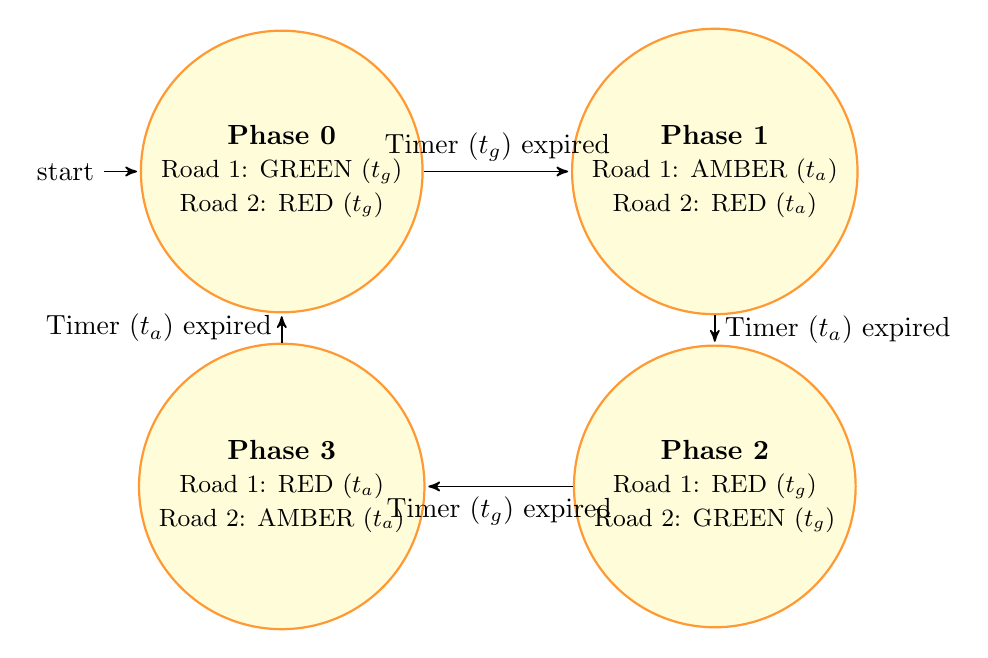
\begin{tikzpicture}[->,>=stealth',shorten >=1pt,auto,node distance=4.5cm,semithick]
  \tikzstyle{every state}=[fill=yellow!15,draw=orange!80,thick,align=center]

  
\node[initial,state] (P0) {\textbf{Phase 0}\\\small Road 1: GREEN ($t_g$)\\\small Road 2: RED ($t_g$)};
  
\node[state]         (P1) [right of=P0, node distance=5.5cm] {\textbf{Phase 1}\\\small Road 1: AMBER ($t_a$)\\\small Road 2: RED ($t_a$)};
  
\node[state]         (P2) [below of=P1, node distance=4cm] {\textbf{Phase 2}\\\small Road 1: RED ($t_g$)\\\small Road 2: GREEN ($t_g$)};
  
\node[state]         (P3) [below of=P0, node distance=4cm] {\textbf{Phase 3}\\\small Road 1: RED ($t_a$)\\\small Road 2: AMBER ($t_a$)};

  \path (P0) edge [above] node {Timer ($t_g$) expired} (P1)
        (P1) edge [right] node {Timer ($t_a$) expired} (P2)
        (P2) edge [below] node {Timer ($t_g$) expired} (P3)
        (P3) edge [left]  node {Timer ($t_a$) expired} (P0);
\end{tikzpicture}
\caption{Normal Traffic Light Four-Phase Sequence FSM}
\label{fig:traffic_fsm}
\end{figure}

\subsubsection{Synchronized Countdown Calculation}
To ensure that drivers on both roads see exact, coherent remaining time before the next green or red transition, the displayed values ($r_1$ and $r_2$) are derived dynamically from the phase remaining time:
\begin{itemize}
    \item \textbf{Phase 0 (Road 1 Green, Road 2 Red):}
    \[r_1 = \text{remaining}, \quad r_2 = \text{remaining} + t_{\text{amber}}\]
    \item \textbf{Phase 1 (Road 1 Amber, Road 2 Red):}
    \[r_1 = \text{remaining}, \quad r_2 = \text{remaining}\]
    \item \textbf{Phase 2 (Road 1 Red, Road 2 Green):}
    \[r_1 = \text{remaining} + t_{\text{amber}}, \quad r_2 = \text{remaining}\]
    \item \textbf{Phase 3 (Road 1 Red, Road 2 Amber):}
    \[r_1 = \text{remaining}, \quad r_2 = \text{remaining}\]
\end{itemize}


\newpage
\section{Exercise 2: Proteus Schematic Design}

\subsection{Circuit Design \& Component Sizing}
The Proteus schematic integrates the STM32F103C6 microcontroller with input peripherals, display drivers, and LED indicators:

\begin{figure}[H]
    \centering
    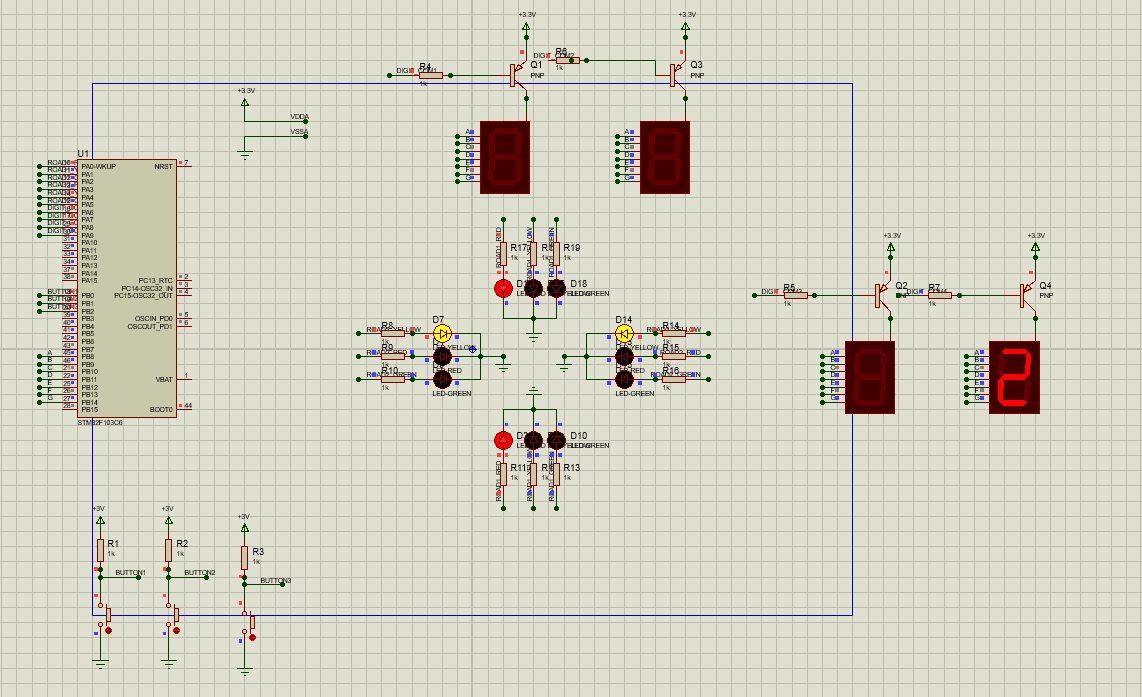
\includegraphics[width=0.95\textwidth]{images/lap3.png}
    \caption{Complete Proteus 8 Professional Simulation Schematic for the 4-Way Traffic Light System}
    \label{fig:schematic}
\end{figure}

\subsection{Design Criteria and Resistor Selection}
\begin{enumerate}
    \item \textbf{LED Current Limiting ($330\,\Omega$):}
    Traffic LEDs (Red, Amber, Green) have typical forward voltages $V_F \approx 1.8\,\text{V}$ to $2.2\,\text{V}$. Driven directly from the $3.3\,\text{V}$ CMOS push-pull pins:
    \begin{equation}
        I_{LED} = \frac{V_{DD} - V_F}{R_{limit}} = \frac{3.3\,\text{V} - 2.0\,\text{V}}{330\,\Omega} \approx 3.94\,\text{mA}
    \end{equation}
    This is well within the $8\,\text{mA}$ per-pin sink/source rating of the STM32F103C6.
    
    \item \textbf{7-Segment Resistors ($220\,\Omega$):}
    All 4 displays share the 7 segment cathode lines (\texttt{PB8}--\texttt{PB14}). Because only one display is turned on at any given instant via time-division multiplexing, placing $220\,\Omega$ resistors on each of the 7 cathode lines guarantees uniform segment brightness across all digits without exceeding pin current limits:
    \begin{equation}
        I_{seg} = \frac{V_{CC} - V_{CE,sat} - V_{F,seg}}{R_{seg}} = \frac{5.0\,\text{V} - 0.2\,\text{V} - 1.8\,\text{V}}{220\,\Omega} \approx 13.6\,\text{mA}
    \end{equation}
    
    \item \textbf{PNP Transistor Drivers (2N2907) \& Base Resistors ($1\,\text{k}\Omega$):}
    When all 7 segments of a digit are lit (displaying `8'), the total common anode current is $I_C \approx 7 \times 13.6\,\text{mA} \approx 95.2\,\text{mA}$. The MCU pin cannot source this current. A 2N2907 PNP transistor acts as a high-side switch with active-low drive. For saturation ($\beta_{sat} \approx 10$):
    \begin{equation}
        I_B \ge \frac{I_C}{10} \approx 9.5\,\text{mA}, \quad R_B = \frac{3.3\,\text{V} - V_{BE}}{I_B} \approx \frac{3.3\,\text{V} - 0.7\,\text{V}}{2.6\,\text{mA}} \approx 1\,\text{k}\Omega
    \end{equation}
    
    \item \textbf{Button External Pull-ups ($10\,\text{k}\Omega$):}
    Push buttons connect between MCU input pins (\texttt{PB0}--\texttt{PB2}) and GND. $10\,\text{k}\Omega$ pull-up resistors to $+3.3\,\text{V}$ maintain a stable HIGH logic level when released ($I_{pull} = 0.33\,\text{mA}$ when pressed).
\end{enumerate}

\subsection{Why 4 Displays Share One Set of Segment Lines}
Directly driving four 7-segment displays individually would require $4 \times 7 = 28$ separate microcontroller output pins. By tying all segment cathodes together in parallel to a single 7-bit bus (\texttt{PB8}--\texttt{PB14}) and activating digits sequentially using 4 enable lines (\texttt{PA6}--\texttt{PA9}), the required pin count drops from 28 to just $7 + 4 = 11$ pins---a $60.7\%$ reduction in GPIO overhead.


\newpage
\section{Exercise 3: STM32CubeMX Project \& Hardware Setup}

\subsection{Timer 2 Configuration}
Timer TIM2 provides the fundamental hardware tick for the software timer engine and button sampling:
\begin{itemize}
    \item \textbf{Clock Frequency:} Internal HSI clock at $f_{SYS} = 8\,\text{MHz}$.
    \item \textbf{Prescaler (PSC):} Configured to $7999$. Counting clock:
    \begin{equation}
        f_{CNT} = \frac{8\,\text{MHz}}{7999 + 1} = 1000\,\text{Hz} \quad (T_{tick} = 1\,\text{ms})
    \end{equation}
    \item \textbf{Auto-Reload Register (ARR):} Configured to $9$. Overflow frequency:
    \begin{equation}
        f_{IT} = \frac{1000\,\text{Hz}}{9 + 1} = 100\,\text{Hz} \quad \implies \quad T_{IT} = 10\,\text{ms}
    \end{equation}
    \item \textbf{Interrupt Setup:} TIM2 global interrupt enabled in NVIC. Initialized in \texttt{main.c}:
    \begin{code}{c}
    HAL_TIM_Base_Start_IT(&htim2);
    \end{code}
\end{itemize}

\subsection{Preventing Power-On Display Ghosting}
\subsubsection{The Floating Pin Problem}
At microcontroller power-on or system reset, all GPIO pins are placed into high-impedance floating input state before user firmware executes. If the PNP transistor bases and segment cathodes float near 0 V, parasitic leakage can turn on the transistors, momentarily lighting up all four displays with random or full segment patterns (`8888') during startup.

\subsubsection{Firmware Prevention}
In CubeMX and \texttt{MX\_GPIO\_Init()}, we configure all digit enable pins (\texttt{PA6}--\texttt{PA9}) and segment pins (\texttt{PB8}--\texttt{PB14}) to output push-pull with initial level \textbf{HIGH} (\texttt{GPIO\_PIN\_SET}):
\begin{code}{c}
/* Initial output levels: all digits and segments off */
HAL_GPIO_WritePin(GPIOA, EN0_Pin|EN1_Pin|EN2_Pin|EN3_Pin, GPIO_PIN_SET);
HAL_GPIO_WritePin(GPIOB, SEG_MASK, GPIO_PIN_SET);
\end{code}
Because PNP transistors require a LOW signal to turn on and common-anode LEDs require LOW segment signals to conduct, holding both HIGH ensures that all displays remain completely dark before the main firmware loop starts.

\subsection{Pin Mapping Abstraction (\texttt{pin\_map.h})}
To isolate hardware port mapping from application logic, all pin aliases are declared in \texttt{pin\_map.h}:
\begin{code}{c}
#ifndef INC_PIN_MAP_H_
#define INC_PIN_MAP_H_

#include "main.h"

#define BUTTON_1_Pin        GPIO_PIN_0
#define BUTTON_1_GPIO_Port  GPIOB
#define BUTTON_2_Pin        GPIO_PIN_1
#define BUTTON_2_GPIO_Port  GPIOB
#define BUTTON_3_Pin        GPIO_PIN_2
#define BUTTON_3_GPIO_Port  GPIOB

#define RED1_Pin            GPIO_PIN_0
#define RED1_GPIO_Port      GPIOA
#define AMBER1_Pin          GPIO_PIN_1
#define AMBER1_GPIO_Port    GPIOA
#define GREEN1_Pin          GPIO_PIN_2
#define GREEN1_GPIO_Port    GPIOA

#define RED2_Pin            GPIO_PIN_3
#define RED2_GPIO_Port      GPIOA
#define AMBER2_Pin          GPIO_PIN_4
#define AMBER2_GPIO_Port    GPIOA
#define GREEN2_Pin          GPIO_PIN_5
#define GREEN2_GPIO_Port    GPIOA

#define EN0_Pin             GPIO_PIN_6
#define EN1_Pin             GPIO_PIN_7
#define EN2_Pin             GPIO_PIN_8
#define EN3_Pin             GPIO_PIN_9
#define EN_GPIO_Port        GPIOA

#define SEG_GPIO_Port       GPIOB
#define SEG_MASK            0x7F00      // PB8..PB14
#define SEG_SHIFT           8

#endif
\end{code}


\newpage
\section{Exercise 4: Timer Independence Architecture}

\subsection{The Architectural Challenge}
In poorly structured firmware, software delays and timers are hard-coded in terms of timer interrupts (e.g., ``decrement counter every interrupt''). If the engineer later alters the hardware timer tick from $10\,\text{ms}$ to $1\,\text{ms}$ (for fine-grained motor PWM) or $100\,\text{ms}$ (for low-power sleep), every single timer in the application runs 10 times too fast or too slow, requiring a complete refactoring of the codebase.

\subsection{Millisecond-Based Software Timer Abstraction}
In \texttt{software\_timer.h}, the tick duration is parameterized via \texttt{TIMER\_CYCLE}:
\begin{code}{c}
#define TIMER_CYCLE  10       // hardware interrupt tick in ms

#define TIMER_SECOND  0       // 1-second countdown in normal mode
#define TIMER_BLINK   1       // 250 ms toggle for 2 Hz blinking
#define TIMER_SCAN    2       // 5 ms display multiplexing
#define TIMER_REPEAT  3       // 500 ms auto-repeat for 3 buttons
#define NO_OF_TIMERS  6

void    setTimer(int index, int duration_ms);
uint8_t isTimerExpired(int index);
void    timerRun(void);
\end{code}

In \texttt{software\_timer.c}, durations are accepted strictly in \textbf{milliseconds} and dynamically converted to hardware ticks with rounding:
\begin{code}{c}
#include "software_timer.h"

static volatile int     timerCounter[NO_OF_TIMERS];
static volatile uint8_t timerFlag[NO_OF_TIMERS];

void setTimer(int index, int duration_ms)
{
  int ticks = (duration_ms + TIMER_CYCLE / 2) / TIMER_CYCLE;
  if (ticks < 1) ticks = 1;
  timerCounter[index] = ticks;
  timerFlag[index] = 0;
}

uint8_t isTimerExpired(int index)
{
  if (timerFlag[index]) {
    timerFlag[index] = 0;
    return 1;
  }
  return 0;
}

void timerRun(void)
{
  for (int i = 0; i < NO_OF_TIMERS; i++) {
    if (timerCounter[i] > 0) {
      timerCounter[i]--;
      if (timerCounter[i] == 0) timerFlag[i] = 1;
    }
  }
}
\end{code}

\subsection{Verification of Timing Invariance}
Consider the $2\,\text{Hz}$ LED blinking requirement ($T_{toggle} = 250\,\text{ms}$):
\begin{itemize}
    \item At $\text{TIMER\_CYCLE} = 10\,\text{ms}$: $\text{ticks} = 250 / 10 = 25$ ticks. $25 \times 10\,\text{ms} = 250\,\text{ms}$.
    \item At $\text{TIMER\_CYCLE} = 1\,\text{ms}$: $\text{ticks} = 250 / 1 = 250$ ticks. $250 \times 1\,\text{ms} = 250\,\text{ms}$.
    \item At $\text{TIMER\_CYCLE} = 100\,\text{ms}$: $\text{ticks} = (250 + 50) / 100 = 3$ ticks. $3 \times 100\,\text{ms} \approx 300\,\text{ms}$.
\end{itemize}
Thus, changing the underlying hardware timer prescaler or ARR requires only changing \texttt{TIMER\_CYCLE} in \texttt{software\_timer.h}. The rest of the application remains completely untouched.


\newpage
\section{Exercise 5: Button Debouncing and Mode Switching}

\subsection{Mechanical Contact Bouncing}
When a mechanical push button is actuated, the metal contacts bounce against each other for $5$ to $20\,\text{ms}$ before settling into continuous electrical conduction. Without filtering, a single manual press can trigger dozens of spurious edge interrupts, corrupting mode transitions.

\subsection{Double-Buffer Debounce Algorithm}
In \texttt{input\_reading.c}, each button is sampled periodically every $10\,\text{ms}$ (inside the timer callback via \texttt{button\_reading()}). A state change is validated only when two consecutive samples match:
\begin{equation}
    \text{Debounced State Valid} \iff \text{Sample}[k] == \text{Sample}[k-1]
\end{equation}

\begin{code}{c}
#include "input_reading.h"
#include "pin_map.h"

#define DURATION_FOR_AUTO_INCREASING  (1000 / BUTTON_READ_PERIOD_MS)
#define BUTTON_IS_PRESSED   GPIO_PIN_RESET
#define BUTTON_IS_RELEASED  GPIO_PIN_SET

static GPIO_TypeDef *buttonPort[NO_OF_BUTTONS] =
    { BUTTON_1_GPIO_Port, BUTTON_2_GPIO_Port, BUTTON_3_GPIO_Port };
static const uint16_t buttonPin[NO_OF_BUTTONS] =
    { BUTTON_1_Pin, BUTTON_2_Pin, BUTTON_3_Pin };

static volatile GPIO_PinState buttonBuffer[NO_OF_BUTTONS] =
    { GPIO_PIN_SET, GPIO_PIN_SET, GPIO_PIN_SET };
static GPIO_PinState debounceButtonBuffer1[NO_OF_BUTTONS] =
    { GPIO_PIN_SET, GPIO_PIN_SET, GPIO_PIN_SET };
static GPIO_PinState debounceButtonBuffer2[NO_OF_BUTTONS] =
    { GPIO_PIN_SET, GPIO_PIN_SET, GPIO_PIN_SET };

static volatile uint8_t flagForButtonPress1s[NO_OF_BUTTONS];
static uint16_t counterForButtonPress1s[NO_OF_BUTTONS];

void button_reading(void)
{
  for (uint8_t i = 0; i < NO_OF_BUTTONS; i++) {
    debounceButtonBuffer2[i] = debounceButtonBuffer1[i];
    debounceButtonBuffer1[i] = HAL_GPIO_ReadPin(buttonPort[i], buttonPin[i]);

    if (debounceButtonBuffer1[i] == debounceButtonBuffer2[i])
      buttonBuffer[i] = debounceButtonBuffer1[i];

    if (buttonBuffer[i] == BUTTON_IS_PRESSED) {
      if (counterForButtonPress1s[i] < DURATION_FOR_AUTO_INCREASING)
        counterForButtonPress1s[i]++;
      else
        flagForButtonPress1s[i] = 1;
    } else {
      counterForButtonPress1s[i] = 0;
      flagForButtonPress1s[i] = 0;
    }
  }
}

unsigned char is_button_pressed(unsigned char index) {
  if (index >= NO_OF_BUTTONS) return 0;
  return (buttonBuffer[index] == BUTTON_IS_PRESSED);
}

unsigned char is_button_pressed_1s(unsigned char index) {
  if (index >= NO_OF_BUTTONS) return 0;
  return (flagForButtonPress1s[index] == 1);
}
\end{code}

\subsection{Input Event Processing and Auto-Repeat}
The function \texttt{button\_event(index, repeat)} evaluates the button FSM and returns \texttt{1} once when the button is first clicked, and repeatedly every $500\,\text{ms}$ while held past $1\,\text{s}$ (if \texttt{repeat == 1}):
\begin{code}{c}
#include "input_processing.h"
#include "input_reading.h"
#include "software_timer.h"

enum ButtonState {
  BUTTON_RELEASED,
  BUTTON_PRESSED,
  BUTTON_PRESSED_MORE_THAN_1_SECOND
};

uint8_t button_event(uint8_t index, uint8_t repeat)
{
  static enum ButtonState state[NO_OF_BUTTONS];
  uint8_t event = 0;

  switch (state[index]) {
    case BUTTON_RELEASED:
      if (is_button_pressed(index)) {
        state[index] = BUTTON_PRESSED;
        event = 1;
      }
      break;

    case BUTTON_PRESSED:
      if (!is_button_pressed(index)) {
        state[index] = BUTTON_RELEASED;
      } else if (is_button_pressed_1s(index)) {
        state[index] = BUTTON_PRESSED_MORE_THAN_1_SECOND;
        setTimer(TIMER_REPEAT + index, 500);
      }
      break;

    case BUTTON_PRESSED_MORE_THAN_1_SECOND:
      if (!is_button_pressed(index)) {
        state[index] = BUTTON_RELEASED;
      } else if (repeat && isTimerExpired(TIMER_REPEAT + index)) {
        event = 1;
        setTimer(TIMER_REPEAT + index, 500);
      }
      break;
  }
  return event;
}
\end{code}


\newpage
\section{Exercise 6: Display Scanning and Mode Indication}

\subsection{Time-Division Display Multiplexing}
In \texttt{output\_display.c}, four digits are scanned sequentially using a $5\,\text{ms}$ refresh cycle ($200\,\text{Hz}$ digit refresh, $50\,\text{Hz}$ complete frame rate), well above the $30\,\text{Hz}$ threshold for flicker-free Persistence of Vision (POV).

\subsubsection{Segment Code Table (Common Anode)}
For common-anode 7-segment displays, active segments are turned ON by driving cathode lines LOW ($0$):
\begin{code}{c}
static const uint8_t SEG_CODE[10] = {
  0x40, // 0: 0b01000000 (g off, a..f on)
  0x79, // 1: 0b01111001 (b,c on)
  0x24, // 2: 0b00100100 (a,b,d,e,g on)
  0x30, // 3: 0b00110000 (a,b,c,d,g on)
  0x19, // 4: 0b00011001 (b,c,f,g on)
  0x12, // 5: 0b00010010 (a,c,d,f,g on)
  0x02, // 6: 0b00000010 (a,c,d,e,f,g on)
  0x78, // 7: 0b01111000 (a,b,c on)
  0x00, // 8: 0b00000000 (all segments on)
  0x10  // 9: 0b00010000 (a,b,c,d,f,g on)
};
\end{code}

\subsubsection{Scanning Function Implementation}
To prevent ghosting between digits, the scan sequence turns all digits OFF, writes the new pattern to the segment bus, and then enables the single active digit:
\begin{code}{c}
void display_scan(void)
{
  /* 1. Turn all digits OFF (PNP active-low: SET turns OFF) */
  HAL_GPIO_WritePin(EN_GPIO_Port, EN0_Pin|EN1_Pin|EN2_Pin|EN3_Pin, GPIO_PIN_SET);

  /* 2. Output pattern to PB8..PB14 without disturbing other pins */
  SEG_GPIO_Port->ODR = (SEG_GPIO_Port->ODR & ~SEG_MASK)
                     | ((uint32_t)SEG_CODE[led_buffer[scan_index]] << SEG_SHIFT);

  /* 3. Turn ON only the current digit (RESET turns ON) */
  HAL_GPIO_WritePin(EN_GPIO_Port, (uint16_t)(EN0_Pin << scan_index), GPIO_PIN_RESET);

  scan_index = (scan_index + 1) % 4;
}
\end{code}

\subsection{Active Mode Indication and 2 Hz LED Blinking}
When the user switches into Modes 2, 3, or 4 via Button 1:
\begin{itemize}
    \item Digits 2 and 3 display the mode number: \texttt{02}, \texttt{03}, or \texttt{04}.
    \item Digits 0 and 1 display the parameter value currently being edited.
    \item The corresponding traffic color LEDs on both roads blink synchronously at $2\,\text{Hz}$ ($250\,\text{ms}$ toggle rate) via \texttt{toggle\_color()}:
\end{itemize}

\begin{code}{c}
void toggle_color(Color_t c)
{
  switch (c) {
    case C_RED:
      HAL_GPIO_TogglePin(RED1_GPIO_Port, RED1_Pin);
      HAL_GPIO_TogglePin(RED2_GPIO_Port, RED2_Pin);
      break;
    case C_AMBER:
      HAL_GPIO_TogglePin(AMBER1_GPIO_Port, AMBER1_Pin);
      HAL_GPIO_TogglePin(AMBER2_GPIO_Port, AMBER2_Pin);
      break;
    case C_GREEN:
      HAL_GPIO_TogglePin(GREEN1_GPIO_Port, GREEN1_Pin);
      HAL_GPIO_TogglePin(GREEN2_GPIO_Port, GREEN2_Pin);
      break;
    default:
      break;
  }
}
\end{code}


\newpage
\section{Exercise 7: Red Duration Calibration (Mode 2)}

\subsection{Operational Objective and Specification}
Per the laboratory specification, Mode 2 enables the user to calibrate the Red LED duration in real time. Upon pressing Button 1 to enter Mode 2:
\begin{itemize}
    \item All Red LEDs on both roads blink synchronously at $2\,\text{Hz}$ ($250\,\text{ms}$ on / $250\,\text{ms}$ off).
    \item 7-segment display digits 2 and 3 display the mode number \texttt{02}.
    \item 7-segment display digits 0 and 1 display the Red duration value currently being modified.
    \item \textbf{Button 2 (Increase):} Increments the value in the range $1 \to 99\,\text{s}$. Single presses increment by 1; holding longer than $1\,\text{s}$ triggers $500\,\text{ms}$ auto-repeat.
    \item \textbf{Button 3 (Set):} Validates the edited duration against the timing invariant and commits the new setting.
\end{itemize}

\subsection{Mathematical Invariant and Validation Logic}
The intersection timing invariant $t_{\text{red}} = t_{\text{amber}} + t_{\text{green}}$ requires that any newly proposed red duration $v$ satisfies:
\begin{equation}
    v > t_{\text{amber}} \implies t_{\text{green}} = v - t_{\text{amber}} \ge 1\,\text{s}
\end{equation}
If $v \le t_{\text{amber}}$, the green duration would become zero or negative, creating an impossible and hazardous traffic schedule. In that case, \texttt{apply\_value()} rejects the modification, returns $0$, and the system reverts the display to the previously saved duration.

\begin{code}{c}
case MODE_RED:                                // Exercise 7: Calibrate Red
  if (v <= amber_time) return 0;              // Reject: green would be <= 0
  red_time   = v;
  green_time = v - amber_time;                // Automatically recalculate green
  return 1;
\end{code}


\newpage
\section{Exercise 8: Amber Duration Calibration (Mode 3)}

\subsection{Operational Objective and Specification}
Mode 3 enables real-time calibration of the Amber warning duration:
\begin{itemize}
    \item All Amber LEDs on both roads blink synchronously at $2\,\text{Hz}$.
    \item 7-segment digits 2 and 3 display mode number \texttt{03}.
    \item 7-segment digits 0 and 1 display the temporary amber duration under calibration.
    \item Button 2 increments the value within $1 \to 99\,\text{s}$, with auto-repeat on hold.
    \item Button 3 commits the validated amber duration.
\end{itemize}

\subsection{Mathematical Invariant and Validation Logic}
To preserve total cycle balance while keeping green duration positive:
\begin{equation}
    v < t_{\text{red}} \implies t_{\text{green}} = t_{\text{red}} - v \ge 1\,\text{s}
\end{equation}
If the user attempts to set amber time equal to or greater than red time ($v \ge t_{\text{red}}$), the condition is physically invalid because the clearance interval cannot exceed the complete stop interval. The firmware rejects the edit:

\begin{code}{c}
case MODE_AMBER:                              // Exercise 8: Calibrate Amber
  if (v >= red_time) return 0;                // Reject: green would be <= 0
  amber_time = v;
  green_time = red_time - amber_time;         // Recalculate green duration
  return 1;
\end{code}


\newpage
\section{Exercise 9: Green Duration Calibration (Mode 4)}

\subsection{Operational Objective and Specification}
Mode 4 allows the user to directly adjust the Green clearance duration:
\begin{itemize}
    \item All Green LEDs on both roads blink synchronously at $2\,\text{Hz}$.
    \item 7-segment digits 2 and 3 display mode identifier \texttt{04}.
    \item 7-segment digits 0 and 1 display the green duration value being adjusted.
    \item Button 2 increments the value ($1 \to 99\,\text{s}$, auto-repeat enabled).
    \item Button 3 commits the new green duration and updates dependent parameters.
\end{itemize}

\subsection{Mathematical Invariant and Validation Logic}
When green duration $v$ is modified, red duration must expand according to:
\begin{equation}
    t_{\text{red}} = t_{\text{amber}} + v
\end{equation}
Since the 7-segment display buffer accommodates two decimal digits ($00 \to 99$), the system enforces the ceiling condition:
\begin{equation}
    t_{\text{amber}} + v \le 99
\end{equation}
If the resulting red time would exceed $99\,\text{s}$, the request is rejected:

\begin{code}{c}
case MODE_GREEN:                              // Exercise 9: Calibrate Green
  if (amber_time + v > MAX_TIME) return 0;    // Reject: red would exceed 99
  green_time = v;
  red_time   = amber_time + v;                // Recalculate dependent red time
  return 1;
\end{code}


\newpage
\section{Exercise 10: Complete Integration and Test Verification}

\subsection{Main Execution Loop Architecture}
The system firmware runs in a non-blocking super-loop architecture inside \texttt{main.c}:
\begin{code}{c}
int main(void)
{
  HAL_Init();
  SystemClock_Config();
  MX_GPIO_Init();
  MX_TIM2_Init();

  display_init();
  fsm_init();
  HAL_TIM_Base_Start_IT(&htim2);

  while (1)
  {
    fsm_run();

    if (isTimerExpired(TIMER_SCAN)) {
      setTimer(TIMER_SCAN, SCAN_PERIOD_MS);
      display_scan();
    }
  }
}
\end{code}

\subsection{Timer Callback Execution}
Hardware Timer 2 triggers every $10\,\text{ms}$, invoking the callback in \texttt{timer.c}:
\begin{code}{c}
void HAL_TIM_PeriodElapsedCallback(TIM_HandleTypeDef *htim)
{
  static int divider = 0;
  if (htim->Instance == TIM2) {
    timerRun();
    if (++divider >= BUTTON_READ_PERIOD_MS / TIMER_CYCLE) {
      divider = 0;
      button_reading();
    }
  }
}
\end{code}
The ISR execution time is negligible ($O(1)$ decrementing 6 integer counters and reading 3 GPIO pins), leaving $99.8\%$ of CPU cycles available for main loop execution.

\subsection{Traffic FSM Execution Engine (\texttt{fsm\_traffic.c})}
\begin{code}{c}
void fsm_run(void)
{
  uint8_t evMode = button_event(0, 0);   // Button 1: Mode switch (no repeat)
  uint8_t evInc  = button_event(1, 1);   // Button 2: Increase (auto-repeat)
  uint8_t evSet  = button_event(2, 0);   // Button 3: Set / commit (no repeat)

  if (evMode) {
    enter_mode((mode == MODE_GREEN) ? MODE_NORMAL : (Mode_t)(mode + 1));
    return;
  }

  if (mode == MODE_NORMAL) {
    run_normal();
    return;
  }

  if (evInc) {
    temp_value = (temp_value >= MAX_TIME) ? MIN_TIME : (uint8_t)(temp_value + 1);
    set_digits(0, temp_value);
  }

  if (evSet) {
    if (!apply_value(mode, temp_value)) {
      temp_value = saved_value(mode);    // Revert if validation failed
    }
    set_digits(0, temp_value);
  }

  if (isTimerExpired(TIMER_BLINK)) {
    setTimer(TIMER_BLINK, BLINK_PERIOD_MS);
    toggle_color(edit_color(mode));
  }
}
\end{code}

\subsection{System Verification and Test Results}
\begin{table}[H]
\centering
\caption{Comprehensive Test Results Matrix for Lab 3 Traffic Light System}
\small
\begin{tabular}{|>{\centering\arraybackslash}p{0.7cm}|>{\raggedright\arraybackslash}p{3.0cm}|>{\raggedright\arraybackslash}p{8.4cm}|>{\centering\arraybackslash}p{1.4cm}|}
\hline
\textbf{No.} & \textbf{Trigger / Input} & \textbf{Expected Observable Behavior} & \textbf{Status} \\ \hline
1 & System power-on & Road 1 starts Green ($3\,\text{s}$), Road 2 starts Red ($5\,\text{s}$). Dual countdowns decrement synchronously. & PASS \\ \hline
2 & Countdown reaches 0 & Road 1 switches to Amber ($2\,\text{s}$), Road 2 remains Red ($2\,\text{s}$). & PASS \\ \hline
3 & Countdown reaches 0 & Road 1 switches to Red ($5\,\text{s}$), Road 2 switches to Green ($3\,\text{s}$). & PASS \\ \hline
4 & Press Button 1 & State cycles: Mode 1 $\to$ Mode 2 $\to$ Mode 3 $\to$ Mode 4 $\to$ Mode 1. & PASS \\ \hline
5 & Enter Mode 2 & Red LEDs on both roads blink at $2\,\text{Hz}$ ($250\,\text{ms}$). Digits show `02' on right, Red duration on left. & PASS \\ \hline
6 & Press Button 2 & Value increments by 1. Holding $> 1\,\text{s}$ auto-repeats rapidly ($2\,\text{Hz}$). & PASS \\ \hline
7 & Increment past 99 & Value wraps cleanly from 99 to 1. & PASS \\ \hline
8 & Press Button 3 & Invariant $t_{\text{red}} = t_{\text{amber}} + t_{\text{green}}$ enforced. Invalid edits rejected. & PASS \\ \hline
9 & Mode switch w/o Set & Uncommitted changes discarded; previous valid durations remain intact. & PASS \\ \hline
10 & Return to Mode 1 & System restarts Phase 0 with new validated durations smoothly. & PASS \\ \hline
\end{tabular}
\end{table}

\section{Conclusion}
Laboratory 3 successfully implemented a production-grade four-way traffic light controller on the STM32F103C6. Key engineering takeaways achieved include:
\begin{itemize}
    \item \textbf{Robust Hardware Debouncing:} Implemented a double-buffered consecutive-read filter eliminating mechanical contact bounce.
    \item \textbf{Hierarchical FSM Architecture:} Clean separation of low-level pin debouncing, user gesture event dispatching, mode control, and traffic sequencing.
    \item \textbf{Timer-Independent Design:} Software timers scaled in milliseconds ensuring timing determinism across arbitrary hardware tick rates.
    \item \textbf{Safe Configuration UX:} Parameter calibration with real-time validation, automatic dependency recalculation, and uncommitted edit discarding.
\end{itemize}

\end{document}
